%
% This file is part of RHexLib, 
%
% Copyright (c) 2001 The University of Michigan, its Regents,
% Fellows, Employees and Agents. All rights reserved, and distributed as
% free software under the following license.
% 
%  Redistribution and use in source and binary forms, with or without
% modification, are permitted provided that the following conditions are
% met:
% 
% 1) Redistributions of source code must retain the above copyright
% notice, this list of conditions, the following disclaimer and the
% file called "CREDITS" which accompanies this distribution.
% 
% 2) Redistributions in binary form must reproduce the above copyright
% notice, this list of conditions, the following disclaimer and the file
% called "CREDITS" which accompanies this distribution in the
% documentation and/or other materials provided with the distribution.
% 
% 3) Neither the name of the University of Michigan, Ann Arbor or the
% names of its contributors may be used to endorse or promote products
% derived from this software without specific prior written permission.
% 
% THIS SOFTWARE IS PROVIDED BY THE COPYRIGHT HOLDERS AND CONTRIBUTORS
% "AS IS" AND ANY EXPRESS OR IMPLIED WARRANTIES, INCLUDING, BUT NOT
% LIMITED TO, THE IMPLIED WARRANTIES OF MERCHANTABILITY AND FITNESS FOR
% A PARTICULAR PURPOSE ARE DISCLAIMED. IN NO EVENT SHALL THE REGENTS OR
% CONTRIBUTORS BE LIABLE FOR ANY DIRECT, INDIRECT, INCIDENTAL, SPECIAL,
% EXEMPLARY, OR CONSEQUENTIAL DAMAGES (INCLUDING, BUT NOT LIMITED TO,
% PROCUREMENT OF SUBSTITUTE GOODS OR SERVICES; LOSS OF USE, DATA, OR
% PROFITS; OR BUSINESS INTERRUPTION) HOWEVER CAUSED AND ON ANY THEORY OF
% LIABILITY, WHETHER IN CONTRACT, STRICT LIABILITY, OR TORT (INCLUDING
% NEGLIGENCE OR OTHERWISE) ARISING IN ANY WAY OUT OF THE USE OF THIS
% SOFTWARE, EVEN IF ADVISED OF THE POSSIBILITY OF SUCH DAMAGE.

%%%%%%%%%%%%%%%%%%%%%%%%%%%%%%%%%%%%%%%%%%%%%%%%%%%%%%%%%%%%%%%%%%%%%%
% $Id: modulemanager.tex,v 1.5 2001/07/19 16:35:56 ulucs Exp $
%
% Created       : Uluc Saranli, 01/06/2001
% Last Modified : Uluc Saranli, 06/27/2001
%
%%%%%%%%%%%%%%%%%%%%%%%%%%%%%%%%%%%%%%%%%%%%%%%%%%%%%%%%%%%%%%%%%%%%%%

\chapter{The Module Manager}
\label{sec:modulemanager}

\section{The \Module\ Class}

In \rhexlib, a {\it Module} is an object which represents a task that needs
to be executed periodically. A template for all such objects is implemented
through the \Module\ virtual base class. All module classes must be derived
from the \Module\ class.

\begin{codesegment}
#include "ModuleManager.hh"
\end{codesegment}

\begin{classdef}
class Module {
protected:
  void setName ( char * str );

public:
  Module( char *name, int index, bool singleUser, bool polling);
  
  char   *getName( void );
  int     getIndex( void );
  MM_STEP getPeriod( void );
  MM_STEP getOffset( void );
  int     getOrder( void );
  Module *getNext( void );
  Module *getPrev( void );
  Module *getOwner( void );
  
  bool    isPolling( void );
  bool    isSingleUser( void );
  
  virtual void init( void ) = 0;
  virtual void uninit( void ) = 0;
  virtual void activate( void ) = 0;
  virtual void deactivate( void ) = 0;
  virtual void update( void ) = 0;
};  
\end{classdef}

\begin{prototype}
Module( char *name, int index, bool singleUser, bool polling);
\end{prototype}

This is the \Module\ constructor. It initializes the module with a given
{\tt name} and {\tt index} which, together, uniquely identify a
module. There cannot be two modules in the system with the same name and
index (see \S\ref{sec:mm_add_remove}). The {\tt singleUser} flag indicates
whether this module can be used by at most one other module at a time or by
many other modules. The {\tt polling} flag indicates that the module will be
updated as frequently as possible. Classes derived from the \Module\ class
are responsible for assigning appropriate values to these arguments in their
constructors.

At any time, a module is in one of three states: {\tt UNINIT}, {\tt
INACTIVE} or {\tt ACTIVE}. Transitions between these states are possible
through module manager functions {\tt MMAddModule()}, {\tt
MMActivateModule()}, {\tt MMDeactivateModule()} and {\tt MMRemoveModule()}
(see \S\ref{sec:mm_info}). The lifecycle of a module, following its
creation, is illustrated in Figure \ref{fig:module_lifecycle}.


%%%%%%%%%%%%%%%%%%%%%%%%%%%%%%%%%%%%%%%%%%%%%%%%
\begin{figure}[ht]
  \begin{center}
    \resizebox{6in}{!}{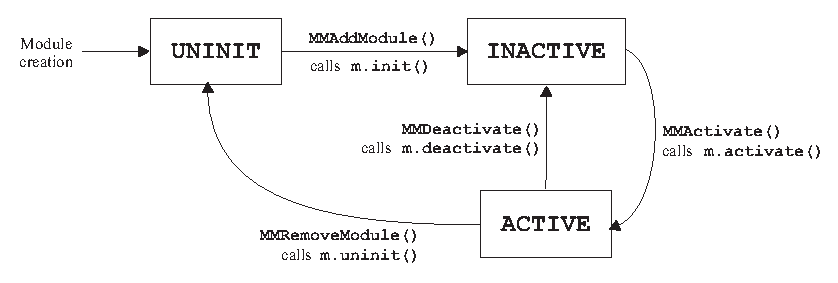
\includegraphics{ModuleLifecycle.eps}}
    \caption{The lifecycle of a module {\tt m}. The boxes represent possible module
      states and the arrows are module manager function calls that affect
      the state of a module.}
    \label{fig:module_lifecycle}
  \end{center}
\end{figure}
%%%%%%%%%%%%%%%%%%%%%%%%%%%%%%%%%%%%%%%%%%%%%%%%


\begin{prototype}
virtual void init( void ) = 0; \\
virtual void uninit( void ) = 0; \\
virtual void activate( void ) = 0; \\
virtual void deactivate( void ) = 0; \\
virtual void update( void ) = 0;
\end{prototype}

These methods define the functionality of a module and are invoked by the
module manager as necessary. The \Module\ base class defines them as pure
virtual functions. It is the responsibility of the programmer to define
these functions in classes derived from the \Module\ base class.

The \initFN\ method is called when a module is ``added'' to the Module
Manager (see \S\ref{sec:mm_add_remove}). Usually, it is only called once. It
should initialize all internal components (i.e.\ allocate memory) and
prepare the module for activation.

The \activateFN\ method is called when the module manager receives a request
to activate a module object. The module manager will start scheduling the
calls to the module's \updateFN\ function once the module has been activated. This
method should initialize all the necessary components of the module,
particularly those that depend on the {\it time} the module was activated,
thereby preparing the \updateFN\ method to be called.

The \updateFN\ method defines the task that the module represents. It is
periodically called by the module manager based on the scheduling parameters
specified at the time the module is added to the system.

The \deactivateFN\ method is called when the module manager receives a
request to deactivate a module object. It should perform any tasks that
depend on the time that the module is deactivated. Following the
deactivation, the module manager will not update the module.

The \uninitFN\ method is called when a module is ``removed'' from the system
(see \S\ref{sec:mm_add_remove}). Usually, it is only called once. It should
clean up all internal components (i.e.\ deallocate memory). The module will
most likely be deleted after this member function is called.

\begin{prototype}
char *getName( void ); \\
int   getIndex( void ); \\
\end{prototype}

These methods are used to access the name and index of a module.

\begin{prototype}
void setName ( char *name );
\end{prototype}
%laura: why do we have this function? it seems useless, and
%potentially dangerous.

This protected method can be used by classes derived from the \Module\ class
to explicitly set the name outside the constructor. However, the name of a
module should, by design, not change after initialization.

\begin{prototype}
\mmstep\ getPeriod( void ); \\
\mmstep\ getOffset( void ); \\
int     getOrder( void );
\end{prototype}

These methods provide access to the period, offset and order parameters of a
module. By definition, the \updateFN\ method of a module is periodically
called (by the Module Manager, see \S\ref{sec:mm_main_loop}) to accomplish the
periodic task the module represents. The {\tt period} and {\tt offset}
parameters determine the periodicity and the beginning time offset of the
first update, respectively. If multiple modules are to be updated in the
same step, the {\tt order} parameter determines the execution order. See
\S\ref{sec:mm_main_loop} for a discussion of module update scheduling.

\begin{prototype}
Module *getNext( void );\\
Module *getPrev( void );
\end{prototype}

The module manager keeps track of all the modules that have been added to it
in one of two linked lists, one for normal modules, the other one for
polling modules. These methods access the next and previous
modules in the list (see \S\ref{sec:mm_add_remove}).
%laura: maybe it would be nice if you explained somewhere why there
%are two linked lists.

\begin{prototype}
Module *getOwner( void );
\end{prototype}

The activation of modules which are configured to be single-user modules
requires the presence of an pointer to an {\it owner} module. The module
manager keeps track of this ownership relation and enforces the single-user
requirement (see \S\ref{sec:mm_activation}). This method returns a pointer
to the current owner of this module or {\tt NULL} if there is no owner at
the time of the call.
%laura: i would mention here that a single-user module does not HAVE
%to have an owner, ie. the pointer to the owner may be NULL.

\begin{prototype}
bool isPolling( void );\\
bool isSingleUser( void );
\end{prototype}

These methods are predicates used to determine if a module is a single-user
and/or a polling module as explained in the constructor function.

\section{The Module Manager}
\label{sec:mm_info}

The \ModuleManager\ class implements a facility to manage all module
activity in the system. The interface to its functionality, however, is not
through its member functions, but through a collection of wrapper
functions. Including the {\tt ModuleManager.hh} file initializes a single
global \ModuleManager\ object. Although the creation of additional
\ModuleManager\ objects is possible, it is not an intended use of the class
and is therefore strongly discouraged. Instead, the global instance
should be used through the wrapper functions described in this section.

The module manager provides many functions for handling modules, accessing
hardware and so on, which are described below. These function are all
prefixed with the letter {\tt MM} and are available by including the {\tt
ModuleManager.hh} file.

\begin{prototype}
\CLOCK\ MMGetStepPeriod( void );
\end{prototype}

This method returns the period of the module manager main loop. The value
returned by this function also corresponds to the real time duration of the
\mmstep\ unit.

\begin{prototype}
\mmstep\ MMGetStepCount( void );
\end{prototype}

This method returns the number of steps that the module manager main loop
has gone through since the beginning of execution. The real time elapsed is
the product of this with the module manager step period.

\section{Choosing and Using The Hardware}
\label{sec:choosing_hardware}

In \rhexlib\, the interface to the low level hardware is accomplished
through the virtual \Hardware\ class (see \S\ref{sec:hardware_class}). To
access critical hardware components such as the real-time clock, the module
manager needs to know about which particular hardware object is to be
used. The function {\tt MMChooseHardware()} is used to inform the module
manager of the hardware object to be used. Once the hardware object is
chosen, the function {\tt MMGetHardware} can be used from within any module
to access the currently chosen hardware object for low level operations.

\section{The Module Manager Main Loop and Module Updates}
\label{sec:mm_main_loop}

\begin{prototype}
void MMMainLoop( void );
\end{prototype}

This function transfers control of a \rhexlib\ program to the module
manager. It never returns and so it should not be called until all modules
to be used have been added to the module manager and the appropriate ones
have been activated. Listing \ref{list:mm_main_loop} shows the basic
functionality of the module manager main loop. The two functions {\tt
updateModules()} and {\tt updatePollingModules()}, called by the main loop
only, determine which modules need their update functions to be called for
normal and polling modules, respectively. Polling modules are updated once
every time the module manager executes the loop. Normal modules, on the
other hand, are statically scheduled for updates based on their parameters.

\begin{codefloat}
\begin{codesegment}
  while ( true ) {
    now = readClock();

    if ( now - clock_mark >= step_period ) {
      while ( now - clock_mark >= step_period )
        clock_mark += step_period;

      updateModules ();
    }
    updatePollingModules ();
  }
\end{codesegment}
\caption{Module manager main loop}
\label{list:mm_main_loop}
\end{codefloat}

The module manager schedules modules at periodic intervals, determined by
the module manager time step (see \S\ref{sec:mm_info}). Listing
\ref{list:mm_update_modules} summarizes the {\tt updateModules()} function,
which updates modules in the appropriate order according to a static
schedule.

\begin{codefloat}
\begin{codesegment}
  m = firstModule;
  while ( m != lastModule ) {

    if ( ( ( current_step - m.getOffset() ) mod m.getPeriod() ) == 0 ) {
      if ( m.getState() == MODULE_ACTIVE)
        current->update();
      m = m.nextModuleInOrder;
    }
  }
\end{codesegment}
\caption{Scheduling of modules in {\tt updateModules()}}
\label{list:mm_update_modules}
\end{codefloat}

\noindent The {\it offset} and {\it period} parameters of a module completely determine its update
schedule. The first update of a module is scheduled {\it offset} steps after
the main loop is invoked. Subsequent updates occur periodically until the
module is deactivated or the module manager shuts down. Note that the
addition and activation times of a module do not affect its update
schedule. Finally, if multiple modules are scheduled for a given step, they
are updated in the increasing order of their {\it order} parameters.

\begin{prototype}
void MMShutdown( void );
\end{prototype}

This function performs a clean shutdown of the module manager. It first
deactivates all the currently active modules and then removes all modules
previously added with the {\tt MMAddModule} function (see
\S\ref{sec:mm_add_remove}). The module objects are not deallocated after
removal.

{\bf Note:} Modules should not directly call this function. Due to the fact that
all modules are removed as a result of this function call, no module update
functions will be called and the module manager loop will run indefinitely.

\begin{prototype}
void MMPowerOff( void );
\end{prototype}

Calls {\tt MMShutdown()} and exits the program. Modules can call this
function to terminate execution (e.g. user interrupt, emergency shutdown
etc.)

% eric: should we say where these functions are called from? otherwise,
% users might think they should call them themselves. 

% uluc: They can call MMPowerOff, but not MMShutdown.
% Actually, I was pondering whether we should just remove MMShutdown() or
% not. I am not entirely happy with the way modules can terminate execution
% for the time being. Maybe we should have a flag or something which will
% exit the module manager loop, at the end of which MMShutdown will be
% called? That look more graceful than just calling MMPowerOff().

%laura: maybe you shouldnt' include MMShutDown in the manual, or else
%include it AFTER MMPowerOff, and make it clear that users should use
%PowerOff.

\section{Adding, Removing and Finding Modules}
\label{sec:mm_add_remove}

\begin{prototype}
void MMAddModule( m, period, offset, order ); \\
Module *m; \\
\mmstep\ period, offset; \\
int order;
\end{prototype}

This function adds the module pointed to by {\it *m} to the current list of
modules with the given {\it period}, {\it offset} and {\it order}
parameters. It calls the \initFN\ method of the module and puts it in the
\ModuleInactive\ state.

\begin{prototype}
void MMRemoveModule( Module *m );
\end{prototype}

This function removes the module pointed to by {\it *m} from the current
list of modules. If the module is active, it is deactivated first, through
{\tt MMRemoveModule()}. Then, the module is removed from the module
manager's list and its \uninitFN function is called.

{\bf Note:} Attempting to remove a module which is in use by another module
generates a fatal error, following which the module manager shuts down and
the program exits after displaying an error message (see
\S\ref{sec:errors}). Details of module ownership are explained in
\S\ref{sec:mm_activation}.

% eric: explain what a fatal error is. 
% uluc: fixed.
%laura: question- just above, did you mean to say it is deactivated 
%first through a call to MMDeactivateModule ?

\begin{prototype}
Module *MMFindModule( char *name, int index );
\end{prototype}

This function returns a pointer to the module with the given name and
index. This is the proper way for a module to locate another module whose
services it requires. It is usually used by a module when it is being added
to the system, i.e.\ from within the module's \initFN\ method.

{\bf Note:} If the specified module has not been previously added, this function
returns {\tt NULL}. Callers should check for this return value and generate
an error if necessary.

% eric: no it doesn't, it returns NULL -- which has to be caught by the user.
% uluc: fixed.

\section{Module Activation, Deactivation and Ownership}
\label{sec:mm_activation}

\begin{prototype}
void MMActivateModule( Module *m );
\end{prototype}

This function puts the module pointed to by {\tt *m} into the \ModuleActive\
state and calls its \activateFN\ function if it was not already in the
\ModuleActive\ state. Following this function call, the \updateFN\ method of
the module's \updateFN\ method will be called by the module manager
according to the module's fixed schedule (see \S\ref{sec:mm_main_loop}).

{\bf Note:} Unless absolutely necessary, {\tt MMGrabModule()} should be used
instead of this function because it keeps track of multiple users for
modules and makes sure modules are not deactivated when they are in use.

% eric: what does static mean?
% uluc: static = fixed, does not change once initialized.

\begin{prototype}
void MMDeactivateModule( Module *m );
\end{prototype}

This function puts the module pointed to by {\tt *m} in the \ModuleInactive\
state and calls its \deactivateFN\ method if it was not already in the
\ModuleInactive\ state. Following this function call, the \updateFN\ method
of the module will not be called until the module is activated again.

{\bf Note:} Unless absolutely necessary, {\tt MMReleaseModule()} should be
used instead of this function because it keeps track of multiple users for
modules and makes sure modules are not deactivated when they are in use.

\begin{prototype}
void MMGrabModule( Module *m, Module *asker );
\end{prototype}

This function is a request to make the module {\tt *asker} become the owner
of the module {\tt *m}. This request is granted if the module does not
already have an owner or the module is not of type {\tt singleUser}. In the
latter case, all grab requests are granted. This function also calls {\tt
MMActivateModule()} in order to activate the module. The module manager
keeps track of a grab count for each module.

This facility is provided to grant exclusive access to modules which use
single-user resources (such as analog outputs). Consequently, upon
activation, all modules should call this function to request ownership for
all the resources they will be using in their updates. It is also good
practice to request ownership for multiple user resources, as it does not
result in any overhead and will ensure proper operation in the future.

% eric: somewhere we should list all the things commonly done in the Module 
% methods, i.e. allocate space, find and grab modules, release modules, etc.
% uluc: How about adding a section: Guidelines for Module design.

{\bf Note:} If the module's {\tt singleUser} flag is true and it is already
owned by another module, this function generates a fatal error, resulting in
the termination of the program. Consequently, the use of {\tt
MMGrabModule()} requires careful design in order to avoid untimely
termination of execution.

% eric: not sure what you mean here.
% uluc: Tried to clarify in the previous Note.

\begin{prototype}
void MMReleaseModule( Module *m, Module *asker );
\end{prototype}

This function releases the ownership of a module. The module is also
deactivated if its grab count reaches zero, meaning that it is not being
used by any other module. Consequently, the grab-release method of
allocating module resources also provides a convenient interface to module
activation and deactivation.

{\bf Note:} If {\tt *m} is owned by some module different than {\tt *asker},
a warning is generated and the module is not released.

\section{Timing Functions}
\index{Timing!functions}

\begin{prototype}
double MMReadTime( void );
\end{prototype}

This function returns the time elapsed in seconds since the invocation of the
program. It uses the {\tt readClock()} method of the low level hardware and
provides a low resolution timing facility.

\begin{prototype}
double MMReadUTime( void );
\end{prototype}

This function returns the time elapsed in seconds since the invocation of
the program at a resolution higher than or equal to that of the {\tt
MMReadClock()} function. It uses the {\tt readUClock()} method of the low
level hardware, and is usually computationally more expensive than its low
resolution counterpart.

\begin{prototype}
\CLOCK\ MMReadClock( void );
\CLOCK\ MMReadUClock( void );
\end{prototype}

These functions are internally used by RHexLib in time computations and
should not be used unless absolutely necessary.

\section{Configuration Facilities}

The \rhexlib module manager keeps a system-wide symbol table for
configuration purposes. Each symbol in the table has a name, which is a
character string, a type (which is either \float\, \floats\, \strings\, or
character string) and a value. As an instantiation of the \SymbolTable\
class, this facility can be used to access system configuration data from
ascii files, avoiding the use of hard coded constants. See
\S\ref{sec:symbol_table} for details on file format and different symbol
types.

\begin{prototype}
void MMReadConfigFile( const char *filename );
\end{prototype}
\index{Configuration files!reading}

This function reads in the specified configuration file into the system
level symbol table.

\begin{prototype}
float MMGetFloatSymbol( const char *name, const float def );
\end{prototype}

This function searches the module manager symbol table for a \float\ typed
symbol with the name {\tt *name}. It returns the value of the symbol. If a
symbol with the given name does not exist or if it has a different type, the
supplied default value is returned.

\begin{prototype}
\floats\ MMGetArraySymbol( const char *name );
\end{prototype}

This function searches the module manager symbol table for a \floats\ typed
symbol with the name {\tt *name}. It returns the value of the symbol in a
\floats\ array. If the symbol with the given name does not exist or has a
different type, an empty array of floats is returned.

\begin{prototype}
strings MMGetStringSymbol( char *name, char *str, char *def );
\end{prototype}

This function searches the module manager symbol table for a string typed
symbol with the name {\tt *name}. It returns the value of the symbol. If a
symbol with the given name does not exist or if it has a different type, the
supplied default value is returned.

%laura: i added this-
\begin{prototype}
void MMGetStrArraySymbol( char *name );
\end{prototype}

This function searches the module manager symbol table for a \strings\ 
typed symbol with the name {\tt *name}. It returns the value of the
symbol in a \strings\ array. If the symbol with the given name does
not exist, of if it has a different type, an empty array of char *s
is returned.

\section{Errors, Warnings and Messages} 
% eric: this section needs to be pointed to from above
% uluc: done.

\label{sec:errors}

The module manager provides several facilities to handle errors and display
warnings and messages. Direct output to {\tt stdout} or {\tt stderr} should
be avoided because they often perturb the real-time performance of the
system. The functions described in this section provide a uniform and
configurable way to handle text output.

Even though the current implementation of these functions simply prints the
messages on the console, future versions will support network
communications, logging to files etc.

\begin{prototype}
void MMFatalError( char *fname, char *msg );
\end{prototype}

This function issues a fatal error and displays a message consisting of the
name of the function supplied in {\tt fname} and the error message in {\tt
msg}. Following the message, it calls {\tt MMPoweroff()} and exits the
program after a clean shutdown of the module manager.

{\bf Note:} A newline is appended at the end of the message text.

\begin{prototype}
void MMWarning( char *fname, char *msg );
\end{prototype}

This function displays a warning message consisting of the name of the
function supplied in {\tt fname} and the warning message in {\tt msg} and
returns.

{\bf Note:} A newline is appended at the end of the message text.

\begin{prototype}
void MMMessage( char *msg );
\end{prototype}

This functon displays the supplied message text and returns. No newline is
appended at the end of the message.

\begin{prototype}
void MMPrintModules( void );
\end{prototype}

This function is mainly for debugging purposes. It displays all the modules
currently maintained by the module manager, together with their state and
parameter information.

